\documentclass{gshs_poster_beamer}
\usepackage{enumitem}
\usepackage{amsmath, amssymb} % equation
\usepackage{kotex} % korean
\usepackage{graphicx} % to use \includegraphics
\graphicspath{{images/}}
\usepackage{siunitx} % SI unit
\usepackage{subcaption}
\setitemize[1]{label={\raise1.25pt\hbox{$\blacktriangleright$}}}
\setitemize[2]{label={\scriptsize\raise1.25pt\hbox{$\blacktriangleright$}}}
\setitemize[3]{label={\raise1.25pt\hbox{$\star$}}}
\setitemize[4]{label={-}}
%\setenumerate[1]{label={\theenumi.}}
%%% title, authors, etc...
\ptitle{천체망원경 모터 포커서 컨트롤러 구동 시스템 개발 및 ASCOM 드라이버 개발\\[0.3em]}
\authorone{곽지성}
\authortwo{정기현}
\teacher{박기현}

\begin{document}
\pagestyle{fancy}
\maketitle
%\vspace{1em} 

\begin{columns}[T]

%% Left Column
\column{0.3\textwidth}


\begin{posterbox}{Abstract}
본 논문에서는 자동 초점 조절 구동 시스템을 자동으로 구현하기 위한 방법을 제안한다. 자동 초점 조절 구동 펌웨어는 기본적으로 arduino를 사용하며 여러 기능들이 존재하여 자유로운 설정이 가능하다. ASCOM 드라이버는 C\# 코딩을 이용하여 컴퓨터로 정보전달이 가능하다. 본 논문에서 제안된 방법은 사람이 손으로 제어하는 것보다 정밀하고 빠르게 천체망원경의 초점을 맞출 수 있도록 편의성을 제공한다.
\end{posterbox}

\vspace{1em}

\begin{posterbox}{Introduction}
\begin{itemize}
	\item 천체망원경의 초점을 사람의 손으로 맞추는 것은 흔들림으로 인하여 쉽지 않다.
	\item 이러한 문제를 해결하기 위하여 'Starizona' 회사에서 자동초점조절 장치인 'Micro Touch'를 개발하였다.
	\item 그러나 이를 사용할 때 여러 가지 불편한 점들이 있고, 가격도 매우 비싸다.
	\item 해결책은 이러한 펌웨어를 더욱 저렴한 가격에 개발하는 것이다.
\end{itemize}
\end{posterbox}

\vspace{1em}

\begin{posterbox}{사용한 물품}
	%  \item item 1
	%    \begin{itemize}
	%      \item subitem 1
	%        \begin{itemize}
	%          \item subsubitem 1
	%            \begin{itemize}
	%              \item subsubsubitem 1
	%              \item subsubsubitem 2
	%            \end{itemize}
	%          \item subsubitem 2
	%        \end{itemize}
	%      \item subitem 2
	%    \end{itemize}
	%  \item item 2
	%\end{itemize}
	\begin{itemize}
		\item 천체망원경
		\begin{itemize}
			\item TEC140 광학계에는 Starlight Instruments에서 제작한 3.5" Feather Touch Focuser가 장착 되어 있다.
			\item Starlight Instruments에서는 3.5" Feather Touch Focuser에 장착할 수 있는 STEPPER MOTOR와 MICRO TOUCH FOCUSING SYSTEM을 제작하여 판매하고 있다.
			\item 모터는 구입한 것을 사용하고 MICRO TOUCH FOCUSING SYSTEM과 같은 기능을 가진 포커서 컨트롤러를 제작하였다.
		\end{itemize}
	\begin{figure}[h]
		\centering
		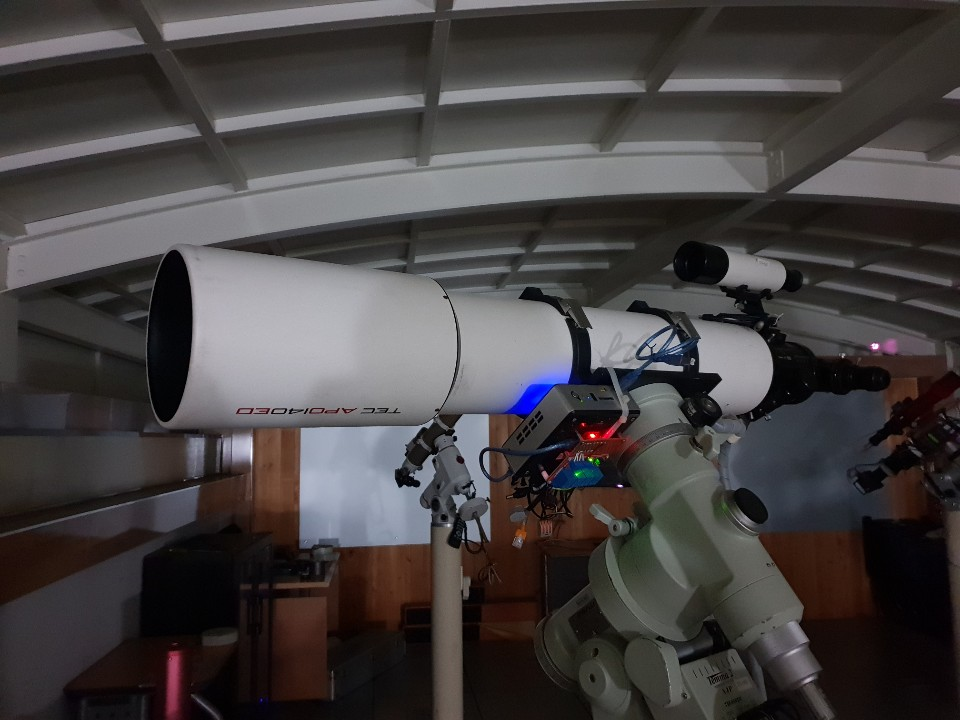
\includegraphics[scale=0.4]{telescope}
		\caption{사용한 천체망원경}
		\label{fig:telescope}
	\end{figure}
		\item arduino
		\begin{itemize}
			\item arduino ARDUINO NANO
			\item 0.96" oled screen I2C
			\item Adafruit Industries 385
			\item Apem MJTP1230B
			\item BP5277-90
			\item HC-05 bluetooth
			\item LED 3mm 90', Ohmite OD473JE
			\item Panasonic EEA-GA1C100H
			\item SparkFun WRL-13678
			\item Sprague 1C10X7R104K050B
			\item TE Connectivity/AMP 5525258-3
			\item TMC2100
			\item Wurth Elektronik 694106301002
		\end{itemize}
	\end{itemize}
	
	%Enumerate
	%\begin{enumerate}
	%  \item item 1
	%    \begin{enumerate}
	%      \item subitem 1
	%        \begin{enumerate}
	%          \item subsubitem 1
	%            \begin{enumerate}
	%              \item subsubsubitem 1
	%              \item subsubsubitem 2
	%            \end{enumerate}
	%          \item subsubitem 2
	%        \end{enumerate}
	%      \item subitem 2
	%    \end{enumerate}
	%  \item item 2
	%\end{enumerate}
	%Description
	%\begin{description}
	%  \item[desc 1] item 1
	%    \begin{description}
	%      \item[desc 1] subitem 1
	%        \begin{description}
	%          \item[desc 1] subsubitem 1
	%            \begin{description}
	%              \item[desc 1] subsubsubitem 1
	%             \item[desc 2] subsubsubitem 2
	%            \end{description}
	%          \item[desc 2] subsubitem 2
	%        \end{description}
	%      \item[desc 2] subitem 2
	%    \end{description}
	%  \item[desc 2] item 2
	%\end{description}
\end{posterbox}


%% Center Column
\column{0.3\textwidth}

\begin{posterbox}{선행연구 고찰}
	\begin{itemize}
		\item 이덕규 외(2014)는 복합재 광구조체와 결합하여 전자광학카메라의 영상품질을 향상시킬 수 있는 초점조절장치를 개발하였다.\cite{leedukgu2014}
		\item 윤종환 외(2011)는 선명도에 관한 기울기를 이용하여 초점이 맞았는지를 확인하는 방법을 사용하였다.\cite{yunjonghwan2011lcd}
		\item 박석휘 외(2009)는 모바일 폰용 자동 초점 조절 알고리즘을 초점 값 계산 알고리즘을 이용하여 구현하였다.\cite{parksukhui2009Median}
		\item 이성희 외(1998)는 각 화소들의 미디언 값의 차이를 이용하여 초점을 맞추는 알고리즘을 구현하였다.\cite{leeseonghee1998Median}
	\end{itemize}
\end{posterbox}

\vspace{1em}

\begin{posterbox}[colbacktitle=black,coltitle=white,colback=black!5]{Bohemian Rhapsody}
  \begin{itemize}
	\item 모터 포커서 컨트롤러 회로 설계
	\begin{figure}[h]
		\centering
		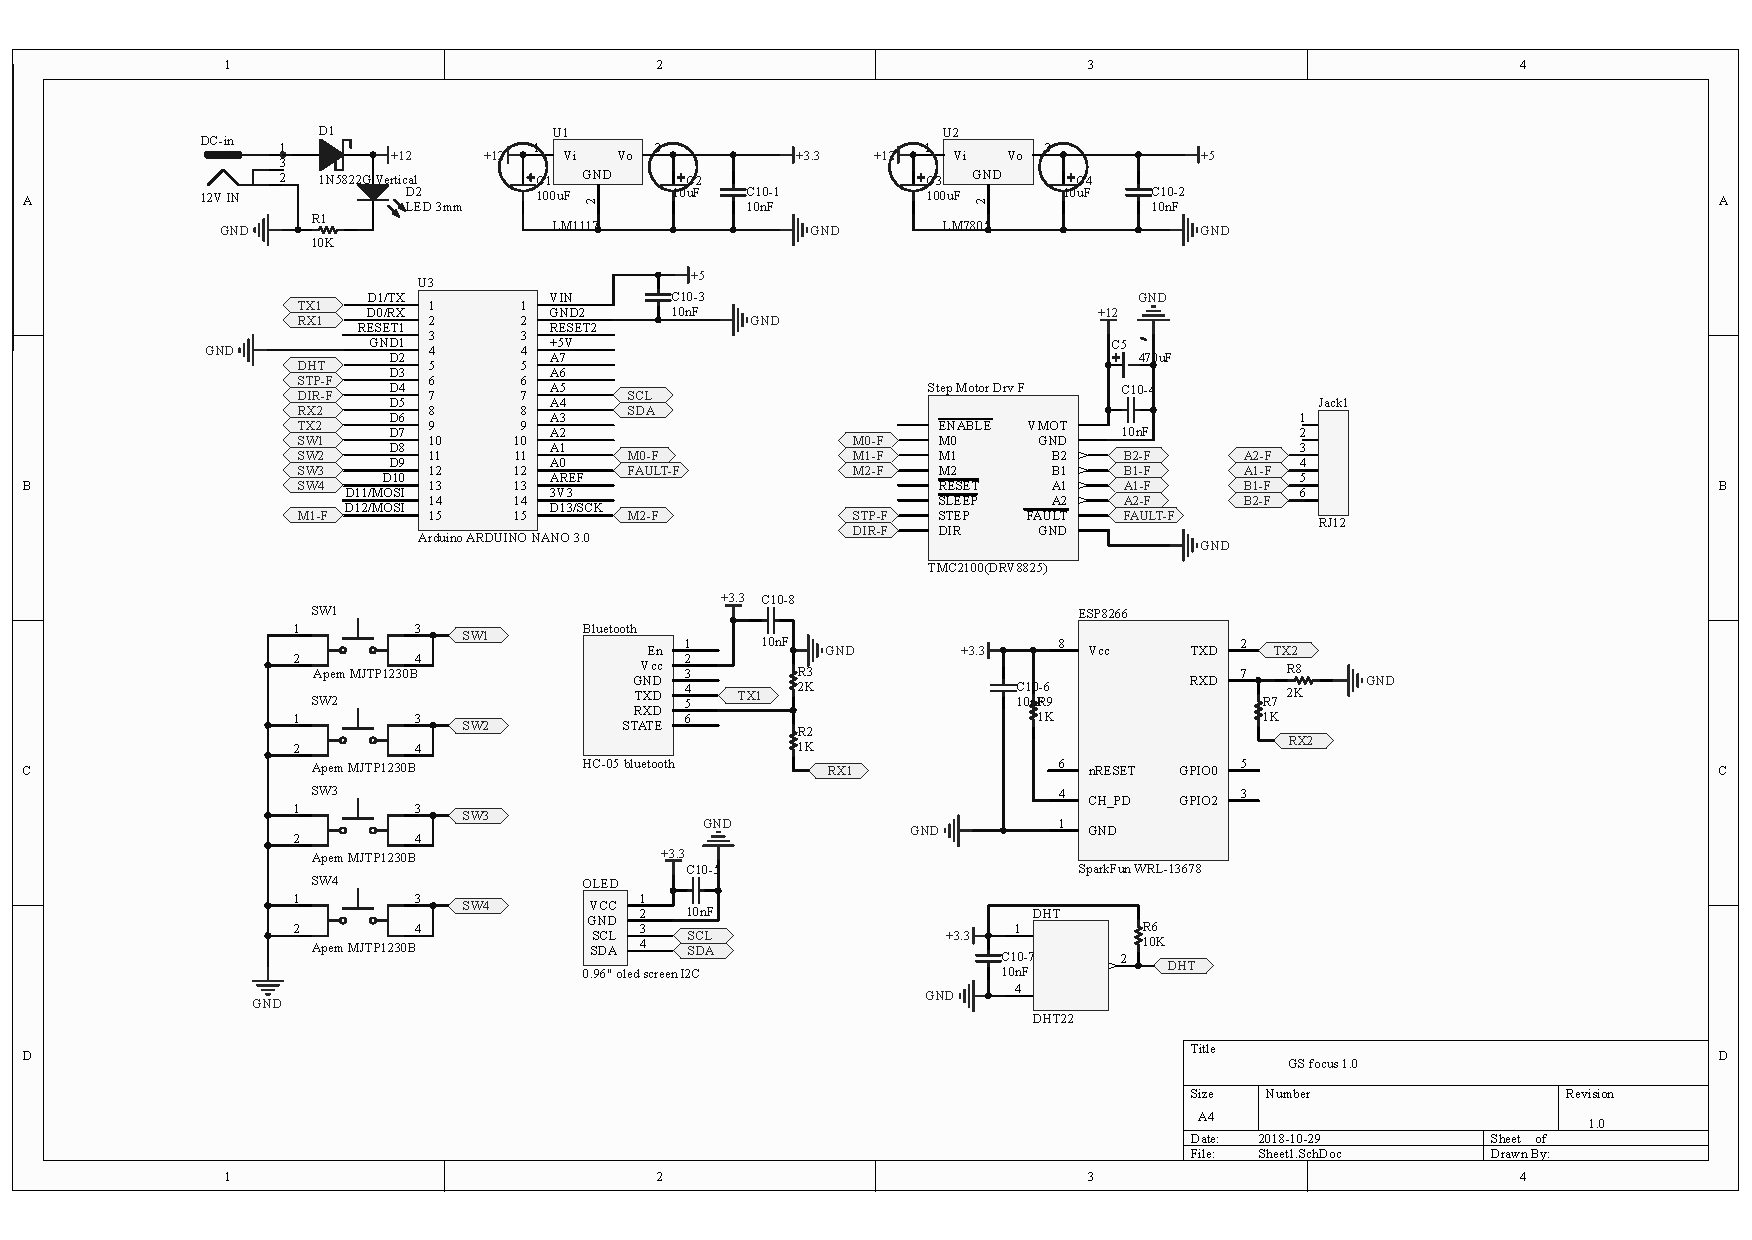
\includegraphics[scale=0.4]{Schematic_Prints}
		\caption{circuitmaker를 이용하여 만든 chart}
		\label{fig:Schematic_Prints}
	\end{figure}
	\begin{figure}[h]
		\centering
		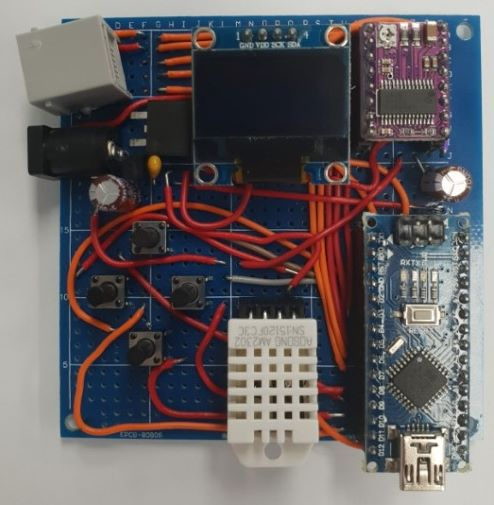
\includegraphics[scale=0.6]{circuit1}
		\caption{만능기판}
		\label{fig:circuit1}
	\end{figure}
	\item 모터 포커서 구동 펌웨어 개발\\
	설계한 회로에 들어갈 펌웨어는 현재 시장에 나와있는 여러 가지 모터포커서에 비해 여러 가지 기능을 지원한다. 먼저, 메뉴 기능을 통해 자신이 원하는 기능을 직접 선택할 수 있도록 하였다. 이를 통하여 모터를 연속적으로 돌리는 기능과 미리 설정한 일정값을 돌릴 수 있도록 지원한다. 특히 연속적으로 돌리는 기능은 버튼을 오래 누를수록 더 빠르게 돌 수 있도록 하여 효율성을 높였다. 또한 모터를 돌리는 것 뿐만이 아니라 자신이 얼마나 돌렸는지 표시하는 기능, 자신이 표시할 숫자를 정하는 기능 등을 포함하고 있다.
	\item ASCOM 드라이버 개발 및 컴퓨터와 연동\\
	모터 자동 초점 조절 장치를 활용하기 위해서는 별의 크기를 분석해서 돌려야 하므로 컴퓨터와의 연동을 위하여 자동 초점 조절 장치의 ASCOM 드라이버를 C\# 코딩을 이용하여 제작한다. ASCOM 드라이버를 이용하면 카메라로부터 정보를 컴퓨터가 받아서 데이터를 분석하고, 이 분석한 데이터를 이용하여 모터를 어떻게 조절해야 할지 명령을 내리면 ASCOM 드라이버를 통해 정보를 전달하여 모터를 제어한 대로 조절이 가능하다.
  \end{itemize}
\end{posterbox}

%% Right Column
\column{0.3\textwidth}
\begin{posterbox}[colbacktitle=blue!50!black,coltitle=white,colback=cyan!5]{연구 결과의 활용과 기대효과}
자동 초점 조절 장치 없이 사람이 직접 초점을 맞추는 것은 정확하지 않고 시간이 많이 든다. 이를 해결하기 위해서 시중에 나온 Micro Touch의 경우 이러한 문제점들을 잘 해결해주고 있다. 하지만 가격이 비싸서 부담스러울 수 있고, 제품을 사용하다보면 길이를 늘이거나 줄일 때 가속기능이 존재하지 않아서 설정되어야 하는 값과 현재 값이 차이가 많이 난다면 설정하는데 시간이 오래 걸린다는 단점이 있다. 본 연구에서는 이러한 단점들을 보완하여 가속기능을 추가하고, arduino 코딩을 기반으로 자동 초점 조절 장치를 개발한다. 이러한 자동 초점 조절 장치가 이용된다면 현재보다 더욱 편리하게 천체망원경의 초점을 맞출 수 있게 되어 천체를 관측하거나 초점을 조절하여 찍은 사진을 이용하는 연구의 경우 사람의 손보다 수월하게 진행이 가능하다.
\end{posterbox}

\vspace{1em}

\begin{posterbox}{추후 연구}
\begin{itemize}
	\item 카메라(또는 CCD) 제어 S/W 개발
	사진 관측을 이용해서 얻은 사진을 컴퓨터로 연결하여 분석이 가능할 수 있도록 만든 카메라(CCD) 제어 시스템을 개발한다. 이를 위하여 사진을 컴퓨터로 보낼 수 있어야 한다. 또한, 카메라에 나오는 화면의 변화를 보아야 하므로 연속적인 변화를 실시간으로 보낼 수 있는 프로그램을 만들어서 컴퓨터가 제대로 인식을 하여 모터에 올바른 명령을 내릴 수 있는지 확인한다.
	\item 오토 포커싱 알고리즘 구현
	천체망원경의 초점을 맞추기 위해 사진 관측의 사진을 연속적으로 찍어서 컴퓨터로 보내주고, 컴퓨터는 이를 분석하여 자동 초점 조절 장치 컨트롤러에 별의 크기가 커지고 있는지 작아지고 있는지 정보를 알고리즘에 보내준다. 그러면 프로그래밍 된 arduino가 모터를 어느 방향으로 돌려야 하는지 판단하여 모터를 돌리고, 이 과정을 반복하여 별의 크기가 제일 작아질 때, 즉 별의 초점이 맞을 때 이 과정을 멈춘다. 이러한 과정이 일어나는지 실제로 천체망원경에 달아서 확인한다.
\end{itemize}
\end{posterbox}

\vspace{1em}

\begin{posterbox}{References}
	
\bibliography{bibfile} % 참고문헌

\end{posterbox}



\end{columns}
\end{document}

